\documentclass[a4paper, 11pt]{article}
\usepackage[top=2cm, bottom=2cm, left=1.5cm, right=1.5cm]{geometry}
\usepackage[utf8]{inputenc}
\usepackage{amsmath, amsfonts, amssymb}
\usepackage{graphicx}
\usepackage[brazil]{babel}
\usepackage{indentfirst}
\usepackage[small,bf]{caption}



\begin{document}
%%%%%%%%%%%%%%%%%%%%%%%%%%%%%%%%Começo do documento%%%%%%%%%%%%%%%%%%%%%%%%


	\begin{enumerate}
	
	\item \textbf{Introdução}
\paragraph{}
O movimento de um corpo em um meio viscoso é influenciado pela ação de uma força viscosa, $F_V$, proporcional à velocidade, $v$. No caso de esferas, assumindo velocidades baixas e um fluido homogêneo e infinito em todas as direções, chega-se a uma força de atrito dada pela lei de Stokes: $F_V = 6 \pi \eta rv$, onde $r$ é o raio da esfera e $\eta$ o coeficiente de viscosidade do meio. Se uma esfera de densidade maior que a de um líquido for solta na superfície do mesmo, no instante inicial a velocidade é zero, mas a força resultante acelera a esfera de forma que sua velocidade vai aumentando. Pode-se verificar que a velocidade aumenta não-uniformemente com o tempo e atinge um valor limite, que ocorre quando a força resultante for nula. As três forças que atuam sobre a esfera estão representadas na Fig. 1 e são, além da força viscosa, o peso da esfera, $P$, e o empuxo, $E$. Igualando a resultante dessas três forças a zero, obtém-se a velocidade limite, $v_L$:

$$ v_L = \dfrac{2}{9} \dfrac{\rho - \rho'}{\eta} g r^2 , $$

onde $\rho$ e $\rho’$ são as densidades da esfera e a densidade do meio, respectivamente, e $g$ é a aceleração da gravidade. A figura abaixo mostra esquematizado as forças que atuam na esfera de aço durante um dado momento de sua trajetória ao longo do tubo de vidro contendo mistura de glicerina e água:

		\begin{figure}[h]
		\centering
		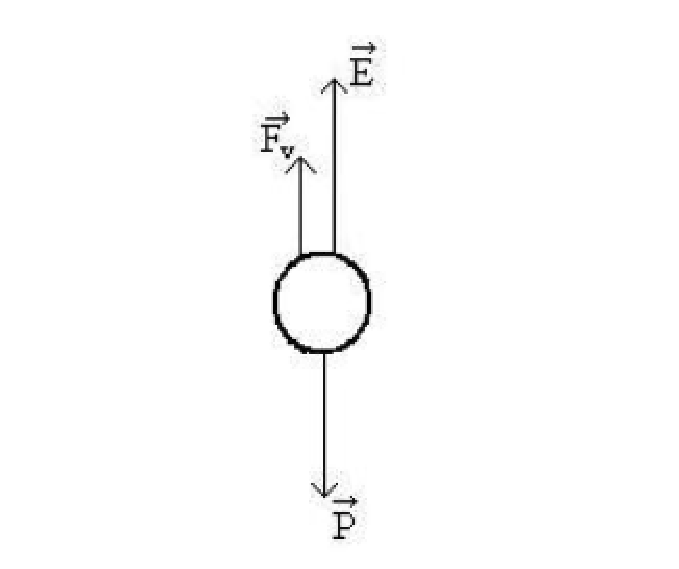
\includegraphics[scale = 0.5]{fig1.eps}
		\caption{Forças que atuam numa esfera num meio viscoso.}
		\end{figure}

\paragraph{}
No experimento dado, como as paredes do tubo de vidro são finitas, logo elas exerceram algum efeito sobre a esfera de aço, alterando a sua velocidade limite, fazendo com que ela não seja exatamente a velocidade da equação $v_L$ dada, então a equação com a correção dessa nova situação é dada da seguinte forma:
$$k \cdot v'_L = \dfrac{2}{9} \dfrac{\rho - \rho'}{\eta} g r^2 ,$$

onde 
$$k = (1 + 2,4 \cdot \dfrac{r}{R})(1 + 3,3 \cdot \dfrac{r}{H})$$
é decorrente do efeito de Ladenburgh, sendo $R$ e $H$, respectivamente, o raio do tubo e a altura total do fluído no tubo. Portanto, temos que multiplicar a velocidade limite da esfera no tubo, $v’_L$, por $k$, para se obter a velocidade limite prevista pela equação de $v_L$.
\pagebreak

	\item \textbf{Materiais necessários}
		\begin{itemize}
		\item Tubo de vidro com mistura de glicerina e água
		\item Suporte com marcas graduadas
		\item Conjunto de esferas
		\item Trena
		\item Paquímetro
		\item Micrômetro
		\item Cronômetro
		\item Termômetro de Aço
		\\
		\end{itemize}

	\item \textbf{Objetivos do Experimento}
		\begin{itemize}
		\item Investigar o movimento de uma esfera de aço em um meio viscoso (mistura de água e glicerina);
		\item Determinar a viscosidade da mistura
		\item Determinar o percentual de água na glicerina
		\\
		\end{itemize}

	\item \textbf{A equação linearizada}
	\paragraph{}
	A equação $v'_L = \dfrac{2}{9} \dfrac{\rho - \rho'}{\eta} g \cdot \dfrac{r^2}{k}$ pode ser linearizada tomando a seguinte relação:
$$ v'_L \longrightarrow y; $$
$$ \dfrac{2}{9} \dfrac{\rho - \rho'}{\eta} g \longrightarrow a $$
$$ \dfrac{r^2}{k} \longrightarrow x $$
que representa uma equação de uma reta do tipo $y = a \cdot x$, teoricamente centrada na origem.
\\

	\item \textbf{Procedimentos para Realização do Experimento}
	\paragraph{}
O primeiro passo é medir o diâmetro de cada uma das esferas com o micrômetro. Para determinar a velocidade limite, nós faremos alguns lançamentos preliminares para determinar uma altura que possa conter o percurso com velocidade constante da esfera afundando na glicerina. Essa altura será medida com uma trena. 
	\paragraph{}
Depois disso, cada membro do grupo fará respectivos lançamentos com cada esfera (de 2 - 3 lançamentos por pessoa por esfera), sempre no centro do tubo – para evitar variações na constante $k$. Um termômetro também precisa estar alocado dentro do tubo, para auxiliar nos resultados finais, que precisam da temperatura do conjunto – assumida constante. Em cada lançamento, o tempo de queda será aferido por um cronômetro digital e, dada a altura e o intervalo de tempo, calcularemos a velocidade limite (que é constante) com $v = \dfrac{\Delta h}{\Delta t}$. 
	\paragraph{}
Essa mesma velocidade também será comparada utilizando o \textit{software} Tracker, a partir de filmagens do experimento, feitas com um celular de um dos membros do grupo. Dados os valores das densidades das esferas de aço e do líquido, bem como o da gravidade, podemos escrever a equação linearizada que é algo da forma \textit{velocidade terminal em função do raio da esfera} – claro, conhecidos os valores dos raios e suas incertezas. Um plot gráfico também será feito para melhor análise. 
	\paragraph{}
Feita a regressão linear, poderemos calcular o valor da viscosidade (que está ligado ao coeficiente angular da reta ajustada) e, conhecidos agora tanto a viscosidade quanto a temperatura, poderemos descobrir qual a concentração de água na nossa glicerina, utilizando o gráfico abaixo, que foi retirado da ref. 5 do roteiro.


		\begin{figure}[!h]
		\centering
		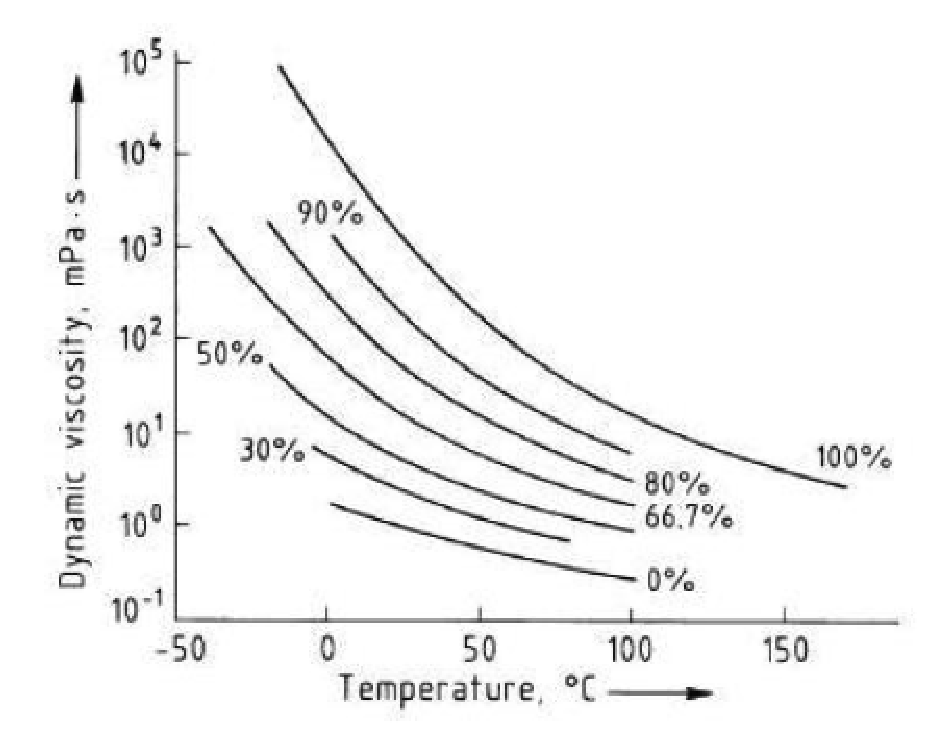
\includegraphics[scale = 0.4]{fig2.eps}
		\caption{Viscosidade da mistura glicerina-água. As concentrações são dadas em percentual de massa de glicerina.}
		\end{figure}

	\paragraph{}
Na falta de uma curva que corresponda adequadamente ao resultado encontrado, mesmo se considerarmos a incerteza do termômetro, podemos supor uma curva intermediária, com um comportamento semelhante ao de suas vizinhas, naquela região. Daí, poderemos tirar o resultado da concentração. Alguns cuidados devem ser tomados para a execução do experimento:
	\begin{itemize}
	\item É recomendado soltar as esferas com velocidade inicial nula (da mesma altura do tubo); 
	\item É importante que se tome cuidado com a separação natural da água e da glicerina, que ocorrerá ao longo do tempo do experimento. Nesse caso, o sistema deixará de ser homogêneo e uma camada de água se formará no topo do tubo. Basta soltar a esfera abaixo dessa camada;
	\item Mais importante: jamais soltar duas bolinhas dentro do tubo. É necessário retirar uma antes de jogar a outra, porque elas podem entupir a válvula e impossibilitar que sejam ambas removidas;
	\item Cuidar para manter sempre o lançamento do centro e da mesma altura, para não modificar o valor da constante do efeito de Ladenburgh.
	\end{itemize}

	\end{enumerate}

%%%%%%%%%%%%%%%%%%%%%%%%%%%%%Fim do documento%%%%%%%%%%%%%%%%%%%%%%%%

\end{document}